\chapter{Domande e (alcune) risposte d'esame}
La maggior parte di questo e del prossimo capitolo è stata spudoratamente scopiazzata dalla mitica \href{http://it.wikipedia.org/wiki/Pagina_principale}{Viky Pedya} (sempre sia lodata), unica e sola fonte di salvezza degli studenti in crisi (e non). Mi sarebbe piaciuto attingere anche da siti più competenti come \href{http://nonciclopedia.wikia.com/wiki/Pagina_principale}{Nonciclopedia}, cui comunque rimando per \href{http://nonciclopedia.wikia.com/wiki/Motore_a_gatto_imburrato}{questo} articolo.


	\section{Domande d'Esame}
\begin{description}[]
	\item[Bernardinello's preface]
Questo documento ha lo scopo di aiutarvi nella preparazione dell'esame. Per superare l'esame è necessario saper rispondere correttamente alle domande che seguono (necessario ma non sufficiente).

Chi ha seguito il corso dovrebbe essere in grado di rispondere alla maggior parte delle domande. Per le domande più nozionistiche, vi è richiesto un piccolo sforzo di ricerca e documentazione. A questo scopo, sfruttate la biblioteca di ateneo; l'Internet è un'altra utile fonte di informazioni, ma va considerata inaffidabile.

Se non vi sentite in grado di rispondere a qualcuna delle domande, stabilite innanzitutto se la questione non è stata trattata a lezione in modo adeguato; in tal caso, segnalatemelo immediatamente.

L'elenco viene di tanto in tanto aggiornato. Tornate a consultarlo.
\newline
\newline
Luca Bernardinello

	

	\item[Fondamenti e Principi dell'Informatica:]\ 
	\begin{enumerate}
		\item
Chi era Alan Mathison Turing (vedi il paragrafo~\vref{subsec:turing})?
		\item
Che cos'è la Macchina di Turing? Che relazione ha con i calcolatori (vedi il paragrafo~\vref{subsec:mturing})?
		\item
Chi era John von Neumann? Descrivere la struttura generale di un calcolatore secondo von Neumann (vedi il paragrafo~\vref{sec:neu}).
		\item
Che cos'è un algoritmo? Dare una definizione il più possibile rigorosa.
	\end{enumerate}
	\item[Architettura dei Calcolatori e Sistemi Operativi:]\ 
	\begin{enumerate}[resume]
		\item
Descrivere la struttura di un calcolatore (vedi il paragrafo~\vref{sec:neu}).
		\item
 Che cos'è un \lstinline!bit!? Che cos'è un \lstinline!byte! (vedi il paragrafo~\vref{susec:bit})?
		\item
Che cos'è un \ac{os}? Quali sono le sue funzioni principali (vedi il paragrafo~\vref{subsec:sis})?
		\item
Come si interagisce con un \ac{os} (vedi il paragrafo~\vref{subsec:inter})?
	\end{enumerate}
	\item[Algoritmica e programmazione:]\ 
	\begin{enumerate}[resume]
		\item
Che cosa si intende per \emph{pseudocodice} (vedi il paragrafo ~\vref{sub:pseudo})?
		\item
Che cos'è un Linguaggio di Programmazione (vedi il paragrafo~\vref{subsec:programmazione})?
		\item
Che cosa si intende per Strutture Dati? Elencate e descrivete qualche struttura di dati dinamica (vedi il paragrafo~\vref{subsec:strutdat}).
		\item
Quali sono le Strutture di Controllo necessarie per esprimere un algoritmo (vedi il paragrafo~\vref{sec:ContStruc})?
		\item
Che cosa si intende per \emph{costo computazionale} di un algoritmo? Come si calcola?
		\item
L'algoritmo di ordinamento \emph{merge sort} ha un costo computazionale asintotico a $O(n\log_2 n)$. Che cosa vuol dire (vedi il paragrafo~\vref{subsec:eff})? (a proposito: che cos'è un algoritmo di ordinamento?)
		\item
Che differenza c'è fra costo computazionale di un algoritmo e costo computazionale di un problema?
		\item
Che cosa si intende per correttezza di un algoritmo? Come possiamo verificare se un algoritmo è corretto?
	\end{enumerate}
\end{description}

\newpage

\section{(Alcune) Risposte d'Esame}
	\subsection{Chi era Alan Mathison Turing?}
	\label{subsec:turing}

		\subsubsection{Introduzione}
\begin{wrapfloat}{figure}{i}{0pt}
	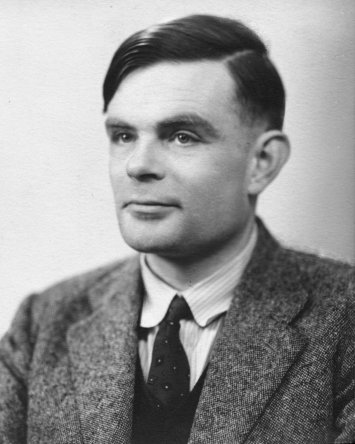
\includegraphics[width=0.6\columnwidth]{immagini/turing_photo}
	\caption[A. M. Turing]{Turing in una foto risalente al 29 Marzo 1951.}
	\label{fig:tur}
\end{wrapfloat}
Alan Mathison Turing (Londra, 23 giugno 1912 -- Wilmslow, 7 giugno 1954) è stato un matematico, logico e crittanalista britannico, considerato uno dei padri dell'informatica e uno dei più grandi matematici del Novecento. Introdusse la macchina ideale e fu anche uno dei più brillanti decrittatori che operavano in Inghilterra durante la seconda guerra mondiale per decifrare i messaggi scambiati da diplomatici e militari delle Potenze dell'Asse.

Omosessuale, morì suicida a soli 42 anni in seguito ad una persecuzione omofobica condotta nei suoi confronti. In suo onore la \ac{acm} ha creato nel 1966 il ""Turing Award'', massima riconoscenza nel campo dell'informatica, dei sistemi intelligenti e dell'intelligenza artificiale.

			\subsubsection{Biografia di Turing}
Turing\marginpar{Nascita} venne concepito in India, durante uno dei viaggi di suo padre, Julius Mathison Turing. Sia Julius che sua moglie, Ethel Sara Stoney, madre del futuro Alan Turing, decisero che il piccolo dovesse nascere sul suolo inglese. Tornarono quindi a Londra dove il 23 Giugno 1912 nacque Alan (figura~\vref{fig:tur}).

Già \marginpar{Infanzia e giovinezza} fin dalla più tenera età, Turing diede segno della genialità. Tuttavia, a causa della sua passione per le materie scientifiche divenne inviso ai professori del St. Michael, la sua prima scuola, i quali avevano sempre posto più enfasi sugli studi classici. Durante i primi anni di scuola ebbe quindi grosse difficoltà, ottenendo a stento il diploma. Poco appassionato al latino e alla religione, preferiva letture riguardanti la teoria della Relatività, i calcoli astronomici, la chimica o il gioco degli scacchi.

Nel\marginpar{Gli anni dell'Università} 1931 venne ammesso al King's College dell'Università di Cambridge dove approfondì i suoi studi sulla meccanica quantistica, la logica e la teoria della probabilità (dimostrò separatamente il \emph{Teorema Del Limite Centrale}, già dimostrato nel 1922 da Lindeberg). Nel 1934 si laureò con il massimo dei voti e nel 1936 vinse il Premio Smith (riconoscimento che veniva assegnato ai due migliori studenti ricercatori in Fisica e Matematica presso l'Università di Cambridge). Nello stesso anno si trasferì alla Princeton University dove studiò per due anni, ottenendo infine un Ph.D. In questi anni pubblicò l'articolo ""On computable Number, with an application to the Entscheidungsproblem'' dove descriveva, per la prima volta, quella che sarebbe poi stata definita come la \emph{macchina di Turing}.

Durante \marginpar{Il lavoro come crittografo} la seconda guerra mondiale, Turing mise le sue capacità matematiche al servizio del \emph{Department of Communications} inglese per decifrare i codici usati nelle comunicazioni tedesche. Con l'entrata in guerra dell'Inghilterra Turing fu ""arruolato'' nel gruppo di crittografi stabilitosi a Bletchley Park e con i suoi compagni lavorò stabilmente. Fu sul concetto di macchina di Turing che nel 1942 il matematico Max Newman progettò una macchina chiamata \emph{Colossus} (antesignana dei computer) che decifrava in modo veloce ed efficiente i codici tedeschi.

Al \marginpar{Il dopoguerra} termine della guerra Turing fu invitato al \ac{npl} a Londra per disegnare il modello di un computer. Il suo rapporto, che proponeva l'\ac{ace}, fu presentato nel marzo 1946 ma ebbe scarso successo a causa degli alti costi preventivati. Per l'anno accademico 1947/48 tornò a Cambridge e spostò i suoi interessi verso la neurologia e la fisiologia. Fu in questo periodo che iniziò ad esplorare la relazione tra i computer e la natura.

Nel \marginpar{Test di Turing} 1950 scrisse un articolo dal titolo ""Computing Machinery And Intelligence'' sulla rivista Mind in cui descriveva quello che sarebbe divenuto noto come il \emph{Test di Turing}. Su questo articolo si basa buona parte dei successivi studi sull'intelligenza artificiale.
L'anno seguente fu eletto Membro della Royal Society di Londra. Si trasferì all'Università di Manchester, dove lavorò alla realizzazione del \ac{madam}. Convinto che entro l'anno 2000 sarebbero state create delle macchine in grado di replicare la mente umana, lavorò alacremente creando algoritmi e programmi per il \ac{madam}, partecipò alla stesura del manuale operativo e ne divenne uno dei principali fruitori.

Nel \marginpar{Reclusione e morte} 1952 sviluppò un approccio matematico all'embriologia. Il 31 marzo dello stesso anno fu arrestato per omosessualità e condotto in giudizio, dove a sua difesa disse semplicemente che "<non scorgeva niente di male nelle sue azioni">. Secondo alcune fonti, Turing avrebbe denunciato per furto un suo amico ospite in casa sua ed ammesso la propria tendenza in risposta a delle domande pressanti della polizia. In quel periodo si dibatteva nel parlamento britannico l'abrogazione del reato di omosessualità e ciò probabilmente avrebbe indotto Turing ad un comportamento incauto. Fu sottoposto alla castrazione chimica, che lo rese impotente e gli causò lo sviluppo del seno; alcuni dei motivi che probabilmente lo condussero, di li a poco, al suicidio.
Nel 1954 Alan Turing morì ingerendo una mela avvelenata con cianuro di potassio, in tono col proprio carattere eccentrico e prendendo spunto dalla fiaba di Biancaneve da lui apprezzata fin da bambino. La madre sostenne che il figlio, con le dita sporche per qualche esperimento chimico, avesse ingerito per errore la dose fatale di veleno; ma il verdetto ufficiale parlò senza incertezze di suicidio:
\begin{quote}
"<Causa del decesso: cianuro di potassio autosomministrato in un momento di squilibrio mentale.">
\end{quote}


	\subsection{Che cos'è un \lstinline!bit!? Che cos'è un \lstinline!byte!?}
	\label{susec:bit}

In informatica, la parola \lstinline!bit! ha due significati molto diversi, a seconda del contesto in cui rispettivamente la si usa:
\begin{itemize}
	\item
\'E l'unità di misura dell'informazione (dall'inglese \emph{binary unit}), definita come la quantità minima di informazione che serve a discernere tra due possibili alternative equiprobabili;
	\item
\'E una \emph{cifra binaria}, (in inglese \emph{binary digit}) ovvero uno dei due simboli del sistema numerico binario, classicamente chiamati zero e uno (0 e 1).
\end{itemize}

Nella \marginpar{Il \lstinline!bit! come quantità d'informazione} prima accezione, un \lstinline!bit! rappresenta l'unità di misura della quantità d'informazione. Intuitivamente, equivale alla scelta tra due valori equiprobabili (sì/no, vero/falso\dots). Matematicamente, la quantità d'informazione in bit di un evento è l'opposto del logaritmo in base due della probabilità (sia essa $p$) di tale evento ($-\log_2 p$). La scelta del numero 2 come base del logaritmo è significativa nel caso elementare di scelta tra due alternative (informazione di un \lstinline!bit!), ma è possibile usare anche $e$ (numero di Nepero), usando dunque il logaritmo naturale ($-\ln p$). In tal caso l'unità di misura dell'informazione si dice \lstinline!Nat!.

Nel caso di due eventi equiprobabili, ognuno ha probabilità $1/2=0,5$. La loro quantità di informazione è, quindi, $-\log_2(1/2) = 1$ \lstinline!bit!.

Nella \marginpar{Il \lstinline!bit! come cifra binaria} seconda eccezione, il \lstinline!bit! rappresenta l'unità di definizione di uno stato logico. La rappresentazione logica del \lstinline!bit! è rappresentata dai soli valori \{$0$, $1$\}. Ai fini della programmazione è comune raggruppare sequenze di \lstinline!bit! in entità più vaste. Questi raggruppamenti contengono generalmente un numero di stringhe binarie pari ad una potenza binaria, pari cioè a $2^n$ con $n \in \mathbb{N} $. Il \marginpar{\emph{Il} byte} più noto è il \lstinline!byte! (chiamato anche \emph{ottetto}), corrispondente ad 8 \lstinline!bit!, che costituisce l'unità di misura più utilizzata in campo informatico.

Altri \marginpar{Altre unità di Misura} raggruppamenti di questo tipo sono i seguenti:
\begin{description}[]
	\item[Nibble:] 4 \lstinline!bit! (1/2 \lstinline!byte!);
	\item[Word:] di lunghezza variabile, corrisponde a 16, 32 o 64 \lstinline!bit!;
	\item[Double Word:] pari a 2 \lstinline!word! (\lstinline!DWORD! o \lstinline!LONGWORD!);
	\item[Quad Word:] pari a 4 \lstinline!word! (\lstinline!QWORD!);
	\item[Kibibyte:] 1024 \lstinline!byte!, indicato con \lstinline!KiB!;
	\item[Mebibyte:] 1024 \lstinline!kibibyte!, indicato con \lstinline!MiB!;
	\item[Gibibyte:] 1024 \lstinline!mebibyte!, indicato con \lstinline!GiB!;
	\item[Tebibyte:] 1024 \lstinline!gibibyte!, indicato con \lstinline!TiB!;
	\item[Pebibyte:] 1024 \lstinline!tebibyte!, indicato con \lstinline!PiB!;
	\item[Exbibyte:] 1024 \lstinline!pebibyte!, indicato con \lstinline!EiB!;
	\item[Zebibyte:] 1024 \lstinline!exbibyte!, indicato con \lstinline!ZiB!;
	\item[Yobibyte:] 1024 \lstinline!zebibyte!, indicato con \lstinline!YiB!.
\end{description}

	\subsection{Che cos'è un \acs{os}? Quali sono le sue funzioni principali?}
	\label{subsec:sis}

I'\ac{os} è un particolare software, installato su un sistema di elaborazione, senza il quale non è possibile l'utilizzo di altri software più specifici (in ultimo, del computer stesso). Esso quindi funge da ""base'' al quale si appoggiano gli altri software, che dovranno essere progettati in modo da essere riconosciuti e supportati da quel particolare sistema operativo. Per \marginpar{Definizione} \ac{os} s'intende dunque l'insieme dei componenti software che hanno il duplice scopo di gestire le risorse hardware e software del computer, ed interfacciare l'utente con l'hardware.

Secondo \marginpar{Funzioni Principali di un \ac{os}} una definizione più rigorosa, il sistema operativo è un insieme di subroutine e strutture dati responsabili di:
\begin{itemize}
	\item
Controllo e della gestione delle componenti hardware che costituiscono il computer (processi di Input/Output da/verso le periferiche collegate al sistema);
	\item
Esecuzione dei programmi che su di esso vengono eseguiti.
\end{itemize}
Se il sistema di elaborazione prevede la possibilità di memorizzazione aggiuntiva dei dati su memoria di massa, ha anche il compito di gestire l'archiviazione e l'accesso ai file. I programmi possono gestire l'archiviazione dei dati su memoria di massa (ottenendo strutture complesse, come un database), servendosi delle procedure messe a disposizione del sistema operativo. La componente dell'\ac{os} che si occupa di tutto ciò viene chiamata \emph{File System}.

Infine, se è prevista interazione con l'utente, viene solitamente utilizzata allo scopo un'interfaccia software (grafica o testuale) per accedere alle risorse hardware del sistema. Solitamente un \ac{os} installato su computer fornisce anche degli applicativi di base per svolgere elaborazioni di diverso tipo.

Al di là delle prestazioni massime offerte dall'hardware dell'elaboratore stesso, l'\ac{os} determina di fatto efficienza e buona parte delle prestazioni effettive di funzionamento dell'intero sistema ad esempio in termini di latenze di processamento, stabilità, interruzioni o crash di sistema.

Un \marginpar{Struttura} generico sistema operativo moderno si compone di alcune parti standard:
\begin{itemize}
	\item
\emph{Kernel}: gruppo di funzioni fondamentali, interconnesse fra loro e con l'hardware, che vengono eseguite con il privilegio massimo disponibile sulla macchina. Il kernel fornisce le funzionalità di base per tutte le altre componenti del sistema operativo, che assolvono le loro funzioni servendosi dei servizi che esso offre;
	\item
\emph{Gestore di File System}: si occupa di esaudire le richieste di accesso alle memorie di massa. Viene utilizzato ogni volta che si accede a un file su disco, e oltre a fornire i dati richiesti tiene traccia dei file aperti, dei permessi di accesso ai file. Inoltre si occupa anche e soprattutto dell'astrazione logica dei dati memorizzati sul computer (directory, ecc);
	\item
\emph{Sistema di Memoria Virtuale}: alloca la memoria richiesta dai programmi e dal sistema operativo stesso, salva sulla memoria di massa le zone di memoria temporaneamente non usate dai programmi e garantisce che le pagine swappate vengano riportate in memoria se richieste;
	\item
\emph{Scheduler}: che scandisce il tempo di esecuzione dei vari processi e assicura che ciascuno di essi venga eseguito per il tempo richiesto;
	\item
\emph{Spooler}: riceve dai programmi i dati da stampare e li stampa in successione, permettendo ai programmi di proseguire senza dover attendere la fine del processo di stampa;
	\item
\emph{Interfaccia utente \emph{(Shell)}}: permette agli esseri umani di interagire con la macchina.
\end{itemize}

	\subsection{Come si interagisce con un \acs{os}?}
	\label{subsec:inter}

Si distinguono due forme d'interazione con un \ac{os}:
\begin{enumerate}
	\item
Interazione gestuale;
	\item
Interazione verbale.
\end{enumerate}
Si parla d'\emph{interazione gestuale}\marginpar{Interazione Gestuale} quando l'utente impartisce comandi al sistema operativo compiendo gesti che sfruttano dispositivi fisici (mouse, tastiera\dots) ed elementi visivi (figurine, menu, finestre\dots). Questa è la forma oggi largamente più diffusa.

Si ha,\marginpar{Interazione Verbale} invece, \emph{interazione verbale} quando i comandi sono impartiti nel corso di un dialogo, sotto forma di parole o sigle. In questo caso l'interazione lascia una traccia su una console, che può occupare l'intero schermo oppure, ed è oggi il caso più frequente, una finestra sullo schermo. Le due forme di interazione possono quindi mescolarsi, e possiamo avere una sessione di interazione verbale nel contesto di un'interazione gestuale. Una \marginpar{Shell} sessione di interazione verbale è governata da un processo, quindi dall'esecuzione di un particolare programma, detto \emph{shell} (cioè ""guscio''). Nei sistemi operativi della famiglia Windows, questo guscio è denominato \emph{prompt dei comandi}. Nei sistemi UNIX, e nei suoi derivati, esistono numerose varianti di shell. Di norma, essa segnala il proprio stato di attesa di comando attraverso un invito (\emph{prompt}, appunto), cioè una particolare sequenza di caratteri visualizzata all'inizio della riga corrente nella console. La forma dell'invito varia da sistema a sistema, e può essere personalizzata da ogni singolo utente.


	\subsection{Che cosa si intende per \emph{pseudocodice}?}
	\label{sub:pseudo}
Per \emph{pseudocodice} (\emph{pseudolinguaggio} o \emph{linguaggio di progetto}) si intende un linguaggio di programmazione fittizio, non direttamente compilabile o interpretabile da un programma compilatore o interprete, il cui scopo è quello di rappresentare algoritmi. Lo pseudolinguaggio può essere utilizzato alternativamente al diagramma di flusso (\emph{flow cahrt}). Lo pseudolinguaggio dipende dal paradigma di programmazione scelto, mentre dovrebbe essere pressoché indipendente dal linguaggio di programmazione, purché quest'ultimo rispetti naturalmente il paradigma scelto.

	\subsection[Cosa si intende per Linguaggio di Programmazione?]{Che cos'è un Linguaggio di Programmazione?}
	\label{subsec:programmazione}

Un \marginpar{Definizione} \emph{linguaggio di programmazione} è un linguaggio formale, dotato di un lessico, di una sintassi e di una semantica ben definiti. È utilizzabile per il controllo del comportamento o la programmazione di una macchina formale attraverso la scrittura di un programma sotto forma di codice. \marginpar{Elementi ""obbligatori''} Tutti i linguaggi di programmazione possiedono:
\begin{itemize}
	\item
\emph{Variabile}: un dato o un insieme di dati, noti o ignoti, già memorizzati o da memorizzare; ad una variabile corrisponde sempre, da qualche parte, un certo numero (fisso o variabile) di locazioni di memoria che vengono allocate per contenere i dati stessi. Molti linguaggi attribuiscono alle variabili un tipo, con differenti proprietà;
	\item
\emph{Istruzione}: un comando o una regola descrittiva. Ogni volta che un'istruzione viene eseguita, lo stato interno del calcolatore cambia.
\end{itemize}
Alcuni \marginpar{Concetti frequenti} concetti sono poi presenti nella gran parte dei linguaggi:
\begin{itemize}
	\item
\emph{Espressione}: una combinazione di variabili e costanti, unite da operatori. Una espressione viene valutata per produrre un valore;
	\item
\emph{Strutture Dati}: meccanismi che permettono di organizzare e gestire dati complessi;
	\item
\emph{Strutture di Controllo}: permettono di governare il flusso d'esecuzione del programma, alterandolo in base al risultato o valutazione di una espressione;
	\item
\emph{Sottoprogramma} (funzione): un blocco di codice che può essere richiamato da qualsiasi altro punto del programma;
	\item
Funzionalità di input di dati da tastiera e visualizzazione dati in output (stampa a video).
\end{itemize}

	\subsection{Che cosa si intende per Strutture Dati? Elencate e descrivete qualche struttura di dati dinamica.}
	\label{subsec:strutdat}

Una \emph{struttura dati} è un'entità usata per organizzare un insieme di dati all'interno della memoria del computer. La scelta delle strutture dati è legata a quella degli algoritmi. Tale scelta, infatti, influisce inevitabilmente sull'efficienza degli algoritmi che la manipolano. La struttura dati è un metodo di organizzazione dei dati, quindi prescinde dai dati effettivamente contenuti.

I linguaggi di programmazione forniscono un insieme predefinito di tipi di dato elementari, e le strutture dati sono strumenti per costruire tipi di dati aggregati più complessi. Esse si differenziano soprattutto in base alle operazioni che si possono effettuare su di esse e alle prestazioni offerte.

		\subsubsection{Costruttori di Strutture Dati}
	
Un \marginpar{Array (o Vettore) [vedi il paragrafo~\vref{subsec:array}]} \emph{Array} è una struttura dati omogenea, che contiene un numero $n$ finito di elementi dello stesso tipo. Questi elementi sono individuati attraverso un indice numerico (da $0$ a $n-1$). La dimensione del vettore deve essere dichiarata al momento della sua creazione.

Un \marginpar{Record (o Struttura) [vedi il paragrafo~\vref{subsec:record}]}  \emph{Record} è una Struttura Dati che può essere eterogenea o omogenea. Nel primo caso contiene una combinazione di elementi che possono essere di diverso tipo. Questi sono detti \emph{campi}, e sono identificati da un nome.

		\subsubsection{Strutture Dati dinamiche}
Le Strutture Dati \emph{dinamiche} sono basate sull'uso di dati di tipo \emph{puntatore} e sull'allocazione dinamica della memoria. Lo spazio di memoria necessario per allocare i puntatori, e le operazioni necessarie alla loro manutenzione costituiscono il \emph{costo aggiuntivo} delle strutture dati dinamiche.

Una \marginpar{Lista Concatenata [vedi il paragrafo~\vref{subsec:liste}]}  \emph{Lista Concatenata} è un insieme di \emph{nodi} collegati linearmente. I nodi sono dei record che contengono un ""carico utile'' di dati, ed un puntatore all'elemento successivo della lista. L'ordine con cui sono collegati i nodi definisce un ordinamento tra di loro. Un nodo funge da testa della lista, e da questo è possibile accedere a tutti i nodi della lista. Conoscendo un nodo interno alla lista, è possibile accedere ai nodi successivi, ma non a quelli precedenti. Il costo di accesso ad un nodo della lista cresce con la dimensione della lista. Conoscendo il nodo precedente ad un nodo N, è possibile rimuovere N dalla lista, o inserire un elemento prima di lui, in un tempo costante.
	
Se \marginpar{Lista Bidirezionale}  la Lista è \emph{bidirezionale}, ogni nodo contiene un puntatore sia al precedente che al successivo. Usando la sintassi del linguaggio C, dato un nodo N il suo successore è \lstinline!N->succ!, e il suo precedente è \lstinline!N->prec!. Deve sempre essere vero che \lstinline!N->succ->prec == N!. Ogni nodo permette di accedere a tutti gli elementi della lista. Gli elementi ``strutturali'' di questa Struttura Dati, ovvero i due puntatori contenuti in ogni nodo, sono ridondanti

Un \marginpar{Alberi [vedi il paragrafo~\vref{subsec:albero}]} \emph{albero} è una rappresentazione dell'albero in teoria dei grafi. Ogni nodo contiene dei puntatori ad altri nodi che sono detti suoi \emph{figli}. Dato un nodo, è possibile accedere a tutti i suoi discendenti. Non deve essere possibile partire da un nodo, seguire i puntatori ai figli e ritornare al nodo di partenza. Inoltre ciascun nodo deve essere figlio di un solo \emph{padre}.

In alcune implementazioni, ogni nodo contiene un collegamento al suo padre. Tra i figli di un nodo esiste normalmente una relazione d'ordine, definita dall'ordine dei puntatori nel padre. In molte implementazioni, ogni nodo ha un numero fissato di figli, ad esempio due o tre. Si parla in questo caso di alberi \emph{binari} o \emph{ternari}. In altri casi, il numero di figli di un nodo è arbitrario.

Gli \marginpar{Binary Search Tree} alberi binari si prestano anche a rappresentare insiemi dotati di ordinamento: un nodo contiene un elemento dell'insieme da ordinare; tutti gli elementi collegati al primo figlio sono precedenti; quelli collegati al secondo sono successivi. Questi   alberi vengono anche definiti \emph{Binary Search Tree} (BST) ovvero alberi di ricerca binaria.
In questo modo, la ricerca di un elemento in un albero ordinato equilibrato richiede un tempo proporzionale al logaritmo del numero di elementi. L'inserimento di un elemento in un albero ordinato richiede di rispettare l'ordinamento precedentemente descritto.

		\subsubsection{Contenitori}
Le strutture dati sopra esposti possono essere utilizzate per realizzare alcuni tipi di \emph{contenitori} di utilizzo frequente, che possono forzare una particolare modalità di accesso ai dati.
	
Il \marginpar{Stack (o Pila) [vedi il paragrafo~\vref{subsec:stack}]} termine \emph{stack} (o pila) viene usato per riferirsi a strutture dati le cui modalità d'accesso seguono una politica LIFO (\emph{Last In First Out}), ovvero tale per cui i dati vengono estratti in ordine rigorosamente inverso rispetto a quello in cui sono stati inseriti. 
	Coda
Per \marginpar{Coda [paragrafo~\vref{subsec:coda}]} \emph{coda}, invece, s'intende una Struttura Dati di tipo FIFO, \emph{First In First Out} (il primo in ingresso è il primo ad uscire). Per implementare una coda viene utilizzato normalmente una Lista Concatenata. La Lista contiene due puntatori uno per la testa (il primo elemento della lista) e uno per la coda (ultimo elemento della Lista).